\section{存在性与版本}
\label{sec:cdis-existence}

正则条件分布要求一个概率核同时给出所有事件的条件概率。逐事件的条件概率总是存在，但每个都只在各自的零概率集之外唯一，拼合时可能出问题。这一节先用一个例子说明随意挑选版本会怎样失败，再给出正则条件分布存在的条件，然后说明它在什么意义下唯一，最后讨论单个零概率观测值上的取值。

\subsection{存在条件}
\label{sec:cdis-existence-conditions}

\paragraph{随意挑选版本的失败}
仍取$Y\sim\operatorname{Unif}(0,1)$、$X=Y$。对每个单点$a\in[0,1]$，事件$\{X=a\}$的概率为零，指示函数几乎必然为零，所以常数$0$是$\mathbb{P}(X=a\mid Y)$的一个合法版本，即可以取$h_{\{a\}}\equiv0$。对每个区间$I$，取$h_{I}(y)=\mathbf{1}_{I}(y)$，这也是合法版本。

现在固定任意一个观测值$y$，看这些版本能否在$y$处拼成一个分布。若概率测度$\mu$在所有区间上满足$\mu(I)=\mathbf{1}_{I}(y)$，则$\mu$与$\delta_y$在区间上相同；区间对有限交封闭并生成Borel集，由测度在生成$\pi$系统上的唯一性，$\mu=\delta_y$，于是$\mu(\{y\})=1$。可是挑出的版本给单点$\{y\}$的值是$0$。这组版本在\emph{每一个}$y$处都拼不成分布，见图~\ref{fig:cdis-version-collapse}。

\begin{BookInlineFigure}
  \centering
  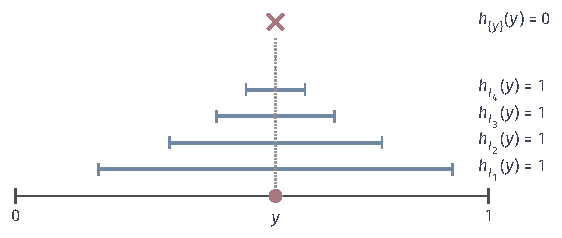
\includegraphics[width=95mm]{figures/07-probability/02-measure-theoretic-probability/tikz/cdis-version-collapse/figure.pdf}
  \caption{随意挑选版本的失败，$X=Y\sim\operatorname{Unif}(0,1)$。固定观测值$y$（红点），包含$y$的区间（蓝线）逐个缩小，所选版本都给出$1$；单点$\{y\}$所选的版本是$0$（红叉）。可数可加性要求区间上的值递减到单点上的值，二者矛盾。}
  \label{fig:cdis-version-collapse}
\end{BookInlineFigure}

每个单点事件的版本只在零概率集$\{Y=a\}$上“出错”，单独看都没有问题；不可数多个这样的零概率集合并起来却覆盖了整个$[0,1]$。补救的思路是：只对可数个事件选版本，可数个零概率集的并仍是零概率集；再用这可数个事件把整个分布确定下来。在实轴上，有理数处的分布函数值就足够确定一个分布。

\paragraph{实值目标}
先处理$X$取实数值的情形。观测$Y$的取值空间不需要任何结构。

\begin{theorem}[实值随机变量的正则条件分布]
\label{thm:cdis-existence-real}
设$X$是实随机变量，$Y$取值于任意可测空间$(\mathcal{Y},\mathcal{F}_{\mathcal{Y}})$。则存在给定$Y$时$X$的正则条件分布，即存在从$\mathcal{Y}$到$(\mathbb{R},\mathcal{B}(\mathbb{R}))$的概率核$K$，使对每个Borel集$A$，$K(Y,A)=\mathbb{P}(X\in A\mid Y)$几乎必然成立。
\end{theorem}

\begin{proof}
证明分四步：在有理数上选版本，收集可数个关系，修正成分布函数，最后核对可测性与版本性质。

第一步，选版本。对每个有理数$q$，由式~\eqref{eq:cdis-function-representation}取可测函数$G_q:\mathcal{Y}\to[0,1]$，使$G_q(Y)=\mathbb{P}(X\leq q\mid Y)$几乎必然。

第二步，收集关系。下面每条都由一个已知结论保证几乎必然成立：
\begin{enumerate}
 \item 对有理数$q<r$，$G_q(Y)\leq G_r(Y)$，由条件期望的保序性；
 \item 对每个有理数$q$，$G_{q+1/n}(Y)\to G_q(Y)$（$n\to\infty$），对递增到$\mathbf{1}_{\{X>q\}}$的$\mathbf{1}_{\{X>q+1/n\}}$用引理~\ref{lem:cdis-conditional-monotone}，再用线性；
 \item $G_{-n}(Y)\to0$，$G_{n}(Y)\to1$（$n\to\infty$），理由同上。
\end{enumerate}
令$N$为使上述某条关系不成立的$y$的全体。每条关系不成立的$y$构成$\mathcal{F}_{\mathcal{Y}}$中的可测集，因为它们由可数个可测函数$G_q$定义；关系几乎必然成立，说明这个集合的$P_Y$测度为零。关系一共可数条，所以$N$可测，并且$P_Y(N)=0$。

第三步，修正。对$y\notin N$，令
\[
 F(t\mid y)=\inf\{G_q(y):q\in\mathbb{Q},\ q>t\},\qquad t\in\mathbb{R}.
\]
由第1条，$F(\cdot\mid y)$不减；作为$q>t$上的下确界，它右连续。由第1、2条，在有理数$q$处$F(q\mid y)=\lim_nG_{q+1/n}(y)=G_q(y)$。由第3条，$t\to-\infty$时$F\to0$，$t\to+\infty$时$F\to1$。所以$F(\cdot\mid y)$是一个分布函数，对应$\mathbb{R}$上唯一的概率测度，记为$K(y,\cdot)$。对$y\in N$，令$K(y,\cdot)=\delta_0$。

第四步，核对。先看可测性。对实数$t$，取有理数$q_n\downarrow t$，则
\[
 K(y,(-\infty,t])=\mathbf{1}_{N^{\mathrm{c}}}(y)\lim_{n\to\infty}G_{q_n}(y)+\mathbf{1}_{N}(y)\,\mathbf{1}_{\{t\geq0\}},
\]
是可测函数的极限与组合，所以可测。使$y\mapsto K(y,A)$可测的Borel集$A$的全体对补集（$K(y,A^{\mathrm{c}})=1-K(y,A)$）和不交可数并（可测函数之和）封闭，含$\mathbb{R}$，是$\lambda$系统；它包含对有限交封闭的半直线族，由$\pi$--$\lambda$定理包含全部Borel集。

再看版本性质。对有理数$q$，在$\{Y\notin N\}$上$K(Y,(-\infty,q])=G_q(Y)$，所以$K(Y,(-\infty,q])=\mathbb{P}(X\leq q\mid Y)$几乎必然。对实数$t$与$q_n\downarrow t$，左边由测度的连续性收敛到$K(Y,(-\infty,t])$，右边由第二步的同一论证几乎必然收敛到$\mathbb{P}(X\leq t\mid Y)$，两者几乎必然相等。使$K(Y,A)=\mathbb{P}(X\in A\mid Y)$几乎必然成立的$A$的全体，由线性与引理~\ref{lem:cdis-eventwise-rules}对补集和不交可数并封闭，同样是含半直线族的$\lambda$系统，于是包含全部Borel集。
\end{proof}

证明的关键在第二步：所有要求都写成可数条，例外集只并了可数次。第三步的下确界把“只在有理数上知道的值”补成右连续的分布函数，在例外集$N$上则直接换成一个固定的分布。图~\ref{fig:cdis-rational-thresholds}用三角形模型画出这两种情形。

\begin{BookInlineFigure}
  \centering
  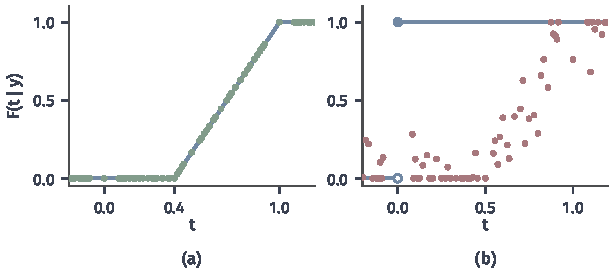
\includegraphics[width=104mm]{figures/07-probability/02-measure-theoretic-probability/matplotlib/cdis-rational-thresholds/figure.pdf}
  \caption{由有理阈值构造条件分布函数（三角形模型）。(a)$y=0.4$不在例外集中：绿点是分母不超过$12$的有理数$q$处的值$G_q(y)$，蓝线是由下确界得到的$F(t\mid y)$，即$[0.4,1]$上均匀分布的分布函数。(b)在一个零概率的观测值上，若所选版本的值（红点）不单调，该点划入例外集，改用固定的分布$\delta_0$（蓝线）。}
  \label{fig:cdis-rational-thresholds}
\end{BookInlineFigure}

\paragraph{标准Borel空间}
证明只用到实轴的两个性质：有一列可数的事件生成全部Borel集，并且在这列事件上相容的值能补成一个测度。许多取值空间可以搬到实轴上而保留这些性质。

\begin{definition}[标准Borel空间]
\label{def:cdis-standard-borel}
可测空间$(\mathcal{X},\mathcal{F}_{\mathcal{X}})$若存在Borel集$S\subseteq\mathbb{R}$与双射$\varphi:\mathcal{X}\to S$，使$\varphi$与$\varphi^{-1}$都可测（$S$取相对Borel $\sigma$代数），则称它为\term{标准Borel空间}（standard Borel space），$\varphi$称为\term{Borel同构}（Borel isomorphism）。
\end{definition}

有限集与可数集（每个子集都可测）满足定义：把元素依次编号为$1,2,\dots$，编号映射与它的逆都可测。更一般地，带Borel $\sigma$代数的完备可分度量空间都是标准Borel空间，其中包括$\mathbb{R}^{d}$、矩阵空间、它们的Borel子集，以及标准Borel空间的可数乘积。这一结论的证明需要用到描述集合论中关于Borel集像的定理，篇幅较长，读者可查阅~\scite{math-kallenberg2021probability}。

它的含义可以从$[0,1)^{2}$看出。把两个坐标写成二进制小数，再把两串数字交替排成一串，就得到$[0,1)$中的一个数，见图~\ref{fig:cdis-digit-interleave}。这个映射把平面上的点一对一地编成一个实数，前$2k$位数字只依赖两个坐标的前$k$位，所以它和它的逆都可测。证明中需要额外处理的只是二进制展开不唯一的那些点，它们构成一个可数集。

\begin{BookInlineFigure}
  \centering
  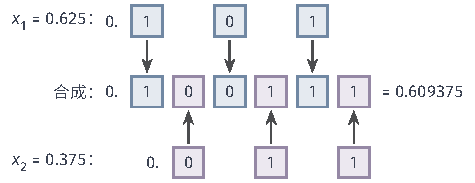
\includegraphics[width=80mm]{figures/07-probability/02-measure-theoretic-probability/tikz/cdis-digit-interleave/figure.pdf}
  \caption{交替排列二进制数字，把$[0,1)^{2}$中的点$(x_1,x_2)$编成$[0,1)$中的一个数。蓝色数字是$x_1=0.625$的二进制位，紫色数字是$x_2=0.375$的二进制位，两串数字$101$与$011$交替排成$100111$，合成的二进制小数$0.100111$等于$0.609375$。}
  \label{fig:cdis-digit-interleave}
\end{BookInlineFigure}

\begin{theorem}[正则条件分布的存在性]
\label{thm:cdis-existence}
设$X$取值于标准Borel空间$(\mathcal{X},\mathcal{F}_{\mathcal{X}})$，$Y$取值于任意可测空间$(\mathcal{Y},\mathcal{F}_{\mathcal{Y}})$，特别地，$\mathcal{Y}$可以是标准Borel空间。则给定$Y$时$X$的正则条件分布存在。
\end{theorem}

\begin{proof}
取Borel同构$\varphi:\mathcal{X}\to S$，令$X'=\varphi(X)$，它是实随机变量。由定理~\ref{thm:cdis-existence-real}，存在给定$Y$时$X'$的正则条件分布$K'$。因为$X'\in S$必然成立，$K'(Y,S)=\mathbb{P}(X'\in S\mid Y)=1$几乎必然，于是集合$N=\{y:K'(y,S)<1\}$可测且$P_Y(N)=0$。

固定一点$x_0\in\mathcal{X}$，令
\[
 K(y,A)=\begin{cases}K'\bigl(y,\varphi(A)\bigr), & y\notin N,\\ \delta_{x_0}(A), & y\in N.\end{cases}
\]
$\varphi(A)=(\varphi^{-1})^{-1}(A)$是$S$的Borel子集，所以右边有意义。$y\notin N$时，$K'(y,\cdot)$的质量全在$S$上，$\varphi$又是双射，$A\mapsto K'(y,\varphi(A))$就是$K'(y,\cdot)$在$S$上的部分经$\varphi^{-1}$推前得到的概率测度。可测性由$K'$继承。最后，$\{X\in A\}=\{X'\in\varphi(A)\}$，所以
\[
 \begin{aligned}
 K(Y,A)&=K'\bigl(Y,\varphi(A)\bigr)=\mathbb{P}\bigl(X'\in\varphi(A)\bigm|Y\bigr)\\
 &=\mathbb{P}(X\in A\mid Y)\quad\text{几乎必然}.
 \end{aligned}\qedhere
\]
\end{proof}

比较一下两种存在性。对单个可积随机变量，条件期望总是存在，第~\ref{chap:conditional-expectation}章用Radon--Nikodym定理构造它，不要求取值空间有任何结构。正则条件分布要把不可数多个条件概率拼在一起，需要目标空间提供一列可数的生成事件以及从这些事件上的值恢复测度的能力；标准Borel条件同时提供了这两点。在没有这类结构的一般可测空间上，可以构造出正则条件分布不存在的例子，构造要用到不可测集，篇幅较长。本卷遇到的取值空间（实数、向量、矩阵、有限或可数的符号集，以及它们的有限或可数乘积）都是标准Borel空间，以后把这一条件作为默认设定，在需要时说明。

\subsection{几乎处处唯一性}
\label{sec:cdis-uniqueness}

正则条件分布找到了一个，是否还有别的？在一个$P_Y$零测集上改动核，积分判别~\eqref{eq:cdis-regular-criterion}察觉不到，问题是除此之外还有没有更大的自由。

\begin{theorem}[正则条件分布的几乎处处唯一性]
\label{thm:cdis-uniqueness}
设$X$取值于标准Borel空间，$K$与$K'$都是给定$Y$时$X$的正则条件分布。则存在$N\in\mathcal{F}_{\mathcal{Y}}$，$P_Y(N)=0$，使对一切$y\notin N$，$K(y,\cdot)=K'(y,\cdot)$。
\end{theorem}

\begin{proof}
先取一个可数且对有限交封闭的事件族$\mathcal{P}$，它生成$\mathcal{F}_{\mathcal{X}}$。$\mathcal{X}=\mathbb{R}$时取$\{(-\infty,q]:q\in\mathbb{Q}\}$；一般情形取Borel同构$\varphi$，令$\mathcal{P}$为这些半直线的原像$\varphi^{-1}((-\infty,q])$的全体，$q\in\mathbb{Q}$。

对每个$P\in\mathcal{P}$，两个核都是$\mathbb{P}(X\in P\mid Y)$的版本，所以$K(Y,P)=K'(Y,P)$几乎必然，即集合$N_P=\{y:K(y,P)\neq K'(y,P)\}$满足$P_Y(N_P)=0$。令$N=\bigcup_{P\in\mathcal{P}}N_P$，它是可数个零测集的并，$P_Y(N)=0$。对$y\notin N$，两个概率测度$K(y,\cdot)$与$K'(y,\cdot)$在生成$\pi$系统$\mathcal{P}$上取值相同，由测度在生成$\pi$系统上的唯一性（可参考\BookChapterRef{chap:measure}{卷四第5章“测度”}），它们在$\mathcal{F}_{\mathcal{X}}$上相同。
\end{proof}

与存在性的证明一样，关键是把比较压缩到可数个事件上，使例外集只并可数次。结论中的例外集用观测的分布$P_Y$来衡量，而不是用$\mathcal{Y}$上的某种“体积”。

\paragraph{单个观测值上的取值}
定理~\ref{thm:cdis-uniqueness}的反面同样重要：联合规律只决定核的$P_Y$等价类，不决定它在某个特定零测点上的值。三角形模型中，把$y=\tfrac12$处的分布换成$\delta_0$，得到核$K'$。$P_Y(\{\tfrac12\})=0$，式~\eqref{eq:cdis-regular-criterion}中积分不受影响，$K'$仍是正则条件分布；可是$K'(\tfrac12,\cdot)$说“给定$Y=\tfrac12$时$X=0$”，而$X\geq Y$本应必然成立。同样可以在所有有理数$y$上改动，甚至在零测的Cantor集上改动。

改动不能扩大到正测度的观测集上。若在$y\in[\tfrac14,\tfrac12]$上把核换成$\operatorname{Unif}(0,1)$，取$A=[0,\tfrac18]$、$B=[\tfrac14,\tfrac12]$。三角形中$X\geq Y\geq\tfrac14$，所以$\mathbb{P}(X\in A,\ Y\in B)=0$，而改动后的核给出
\[
 \int_{1/4}^{1/2}\frac18\cdot2(1-y)\,\mathrm{d}y=\frac14\int_{1/4}^{1/2}(1-y)\,\mathrm{d}y=\frac14\cdot\frac{5}{32}=\frac{5}{128}>0 ,
\]
式~\eqref{eq:cdis-regular-criterion}不成立。图~\ref{fig:cdis-two-versions}对照了两种改动。

\begin{BookInlineFigure}
  \centering
  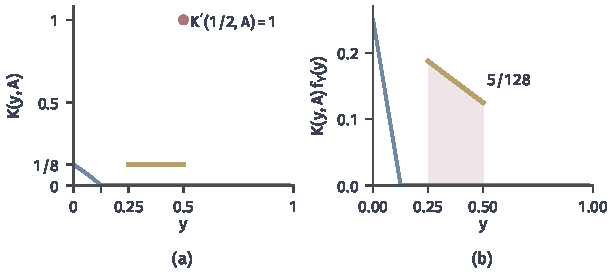
\includegraphics[width=104mm]{figures/07-probability/02-measure-theoretic-probability/matplotlib/cdis-two-versions/figure.pdf}
  \caption{三角形模型中$A=[0,\tfrac18]$时核的几种取法。(a)蓝线是由密度比得到的$y\mapsto K(y,A)$，在$y\geq\tfrac18$时为零；红点是只在$y=\tfrac12$一个点上的改动，它仍给出正则条件分布；黄线把$[\tfrac14,\tfrac12]$整段改成$\tfrac18$。(b)式~\eqref{eq:cdis-regular-criterion}中的被积函数$K(y,A)f_Y(y)$：单点改动不影响积分，黄线的改动多出浅红区域的质量$\tfrac{5}{128}$，不再是正则条件分布。}
  \label{fig:cdis-two-versions}
\end{BookInlineFigure}

若某个观测值本身有正概率，$P_Y(\{y_0\})>0$，它不可能落在零测例外集中，$K(y_0,\cdot)$就被唯一确定，并且由式~\eqref{eq:cdis-regular-criterion}取$B=\{y_0\}$，
\[
 K(y_0,A)=\frac{\mathbb{P}(X\in A,\ Y=y_0)}{\mathbb{P}(Y=y_0)},
\]
这正是第~\ref{chap:classical-probability}章的条件概率。正则条件分布在有正概率的观测值上与初等条件概率一致，额外的自由只出现在零概率的观测值上。

\subsection{零概率条件}
\label{sec:cdis-zero-probability}

$Y$连续时，每个单点的概率都是零，$\mathbb{P}(X\in A\mid Y=y)$不能写成两个事件概率之比。正则条件分布给这个记号一个意义：它就是$K(y,A)$，作为$y$的函数在$P_Y$几乎处处的意义下由联合规律确定。下面先说明密度公式给出一个版本，再讨论单个零概率观测值上附加的选择。

\paragraph{密度公式给出的版本}
设$\alpha,\beta$分别是$\mathcal{X},\mathcal{Y}$上的$\sigma$有限测度，例如Lebesgue测度或计数测度，$(X,Y)$关于乘积测度$\alpha\otimes\beta$有联合密度$f$。记$f_Y(y)=\int f(x,y)\,\alpha(\mathrm{d}x)$为$Y$关于$\beta$的密度。

\begin{theorem}[条件密度给出的正则条件分布]
\label{thm:cdis-density-version}
在上述设定下，任取$\mathcal{X}$上的概率测度$\nu_0$，令
\begin{equation}
 K(y,A)=\begin{cases}
 \dfrac{1}{f_Y(y)}\displaystyle\int_{A}f(x,y)\,\alpha(\mathrm{d}x), & 0<f_Y(y)<\infty,\\
 \nu_0(A), & \text{其他}.
 \end{cases}
 \label{eq:cdis-density-version}
\end{equation}
则$K$是给定$Y$时$X$的正则条件分布。
\end{theorem}

\begin{proof}
对$0<f_Y(y)<\infty$的$y$，$K(y,\cdot)$是非负函数$f(\cdot,y)/f_Y(y)$关于$\alpha$的不定积分，总量为$1$，是概率测度；其余$y$处是$\nu_0$。由Tonelli定理，$y\mapsto\int_{A}f(x,y)\,\alpha(\mathrm{d}x)$与$f_Y$都可测，集合$\{0<f_Y<\infty\}$可测，所以$K(\cdot,A)$可测，$K$是概率核。

再核对式~\eqref{eq:cdis-regular-criterion}。$\int f_Y\,\mathrm{d}\beta=1$，所以$\{f_Y=\infty\}$是$\beta$零测集；$\{f_Y=0\}$上被积函数含因子$f_Y=0$。于是这两部分都不贡献，
\[
 \begin{aligned}
 \int_{B}K(y,A)\,f_Y(y)\,\beta(\mathrm{d}y)&=\int_{B}\int_{A}f(x,y)\,\alpha(\mathrm{d}x)\,\beta(\mathrm{d}y)\\
 &=\mathbb{P}(X\in A,\ Y\in B).
 \end{aligned}
\]
由引理~\ref{lem:cdis-regular-criterion}，$K$是正则条件分布。
\end{proof}

定理同时涵盖了概率表（$\alpha,\beta$都取计数测度）、条件密度（都取Lebesgue测度），以及离散状态与连续读数的混合模型（一个取计数测度，一个取Lebesgue测度）。证明没有用到标准Borel条件：有了联合密度，核可以直接写出来。

公式~\eqref{eq:cdis-density-version}在每个$y$处都给出一个值，但这个值依赖所选的密度$f$。联合密度只在$\alpha\otimes\beta$零测集之外确定；在直线$\{y=y_0\}$上任意改动$f$，联合规律不变，$K(y_0,\cdot)$却变了。单个零概率观测值上的条件分布需要额外的要求来选定。

\paragraph{连续性的要求}
常用的要求是连续性。第~\ref{chap:random-vectors}章证明：若联合密度在$y_0$附近连续且$f_Y(y_0)>0$，窄带$\{y_0\leq Y\leq y_0+h\}$上的条件概率在$h\to0$时趋于密度比。这个极限选出了一个特定的值。设$\mathcal{Y}=\mathbb{R}$。若两个版本对定理~\ref{thm:cdis-uniqueness}证明中可数生成族的每个事件$P$，$y\mapsto K(y,P)$都在$y_0$处连续，并且$y_0$的每个邻域都有正的$P_Y$质量，那么两个版本在$y_0$处相同：它们在一个$P_Y$零测集之外相等，每个邻域里都有这样的点，取极限即得两者在每个$P$上的值相同，再由生成$\pi$系统上的唯一性得到$K(y_0,\cdot)$相同。

这种选择有两个限度。其一，满足要求的版本未必存在。设$Y\sim\operatorname{Unif}(-1,1)$，$X=\mathbf{1}_{\{Y>0\}}$。正则条件分布在$y<0$时是$\delta_0$，在$y>0$时是$\delta_1$（几乎处处唯一），$y=0$处无论取什么，$y\mapsto K(y,\{1\})$都不连续，见图~\ref{fig:cdis-no-continuous}。连续性在这里无法选出$K(0,\cdot)$，这一点的值只能另作约定。

\begin{BookInlineFigure}
  \centering
  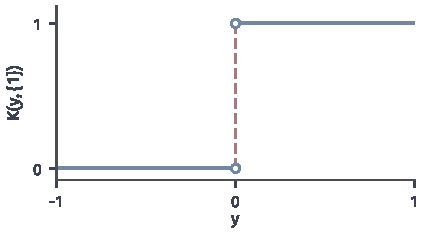
\includegraphics[width=72mm]{figures/07-probability/02-measure-theoretic-probability/matplotlib/cdis-no-continuous/figure.pdf}
  \caption{$Y\sim\operatorname{Unif}(-1,1)$、$X=\mathbf{1}_{\{Y>0\}}$时的$y\mapsto K(y,\{1\})$。蓝线在$y<0$时为$0$，在$y>0$时为$1$；$y=0$处（红色虚线上的任何值）怎样取都不能使它连续。}
  \label{fig:cdis-no-continuous}
\end{BookInlineFigure}

其二，选出的值依赖用哪个观测量逼近同一个零概率事件。设$(X,Y)$在单位正方形上均匀分布，问“给定$X=Y$时$X$的分布”。事件$\{X=Y\}$可以写成$\{D=0\}$，其中$D=Y-X$；也可以写成$\{R=1\}$，其中$R=Y/X$。两种写法描述同一条对角线，给出的条件分布却不同。

\paragraph{两种逼近的计算}
先用$D$。由换元$(x,y)\mapsto(x,d)=(x,y-x)$，Jacobian行列式为$1$，$(X,D)$的联合密度是
\[
 f_{X,D}(x,d)=1,\qquad 0<x<1,\ 0<x+d<1 .
\]
在$d=0$处它对$x\in(0,1)$恒为$1$，边缘$f_D(0)=1$，由式~\eqref{eq:cdis-density-version}，给定$D=0$时$X$的条件密度是$1$，即$X\sim\operatorname{Unif}(0,1)$。

再用$R$。由换元$(x,y)\mapsto(x,r)=(x,y/x)$，逆变换$y=rx$的Jacobian行列式为$x$，$(X,R)$的联合密度是
\[
 f_{X,R}(x,r)=x,\qquad 0<x<1,\ 0<rx<1 .
\]
在$r=1$处它是$x$，边缘$f_R(1)=\int_0^1x\,\mathrm{d}x=\tfrac12$，所以给定$R=1$时$X$的条件密度是$2x$。两个结果都由连续的联合密度得到，都是各自观测量下“连续性选出的”版本，却互不相同。

图~\ref{fig:cdis-borel-kolmogorov}说明差别从哪里来。$\{\lvert D\rvert\leq h\}$是沿对角线等宽的带子，各处收进同样多的质量；$\{\lvert R-1\rvert\leq h\}$是从原点张开的楔形，离原点越远越宽，收进的质量与$x$成正比。两种窄化在极限下落在同一条线上，但沿线分配质量的权重不同。这一现象称为\term{Borel--Kolmogorov悖论}（Borel--Kolmogorov paradox）。

\begin{BookInlineFigure}
  \centering
  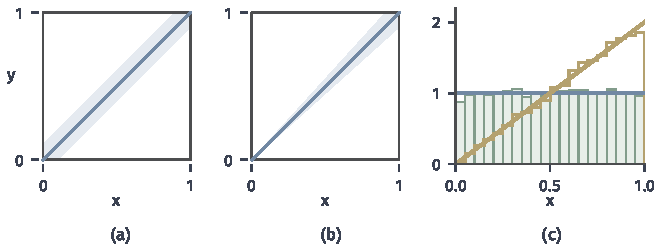
\includegraphics[width=112mm]{figures/07-probability/02-measure-theoretic-probability/matplotlib/cdis-borel-kolmogorov/figure.pdf}
  \caption{同一条对角线的两种逼近，$(X,Y)$在单位正方形上均匀分布。(a)浅蓝带子$\{\lvert Y-X\rvert\leq h\}$，$h=0.1$。(b)浅蓝楔形$\{\lvert Y/X-1\rvert\leq h\}$，$h=0.1$。(c)固定种子$7$模拟$4\times10^{5}$个点，取$h=0.02$：落在带子中的点的$X$坐标直方图为浅绿柱，落在楔形中的为黄色阶梯线；蓝线与黄线是极限密度$1$与$2x$。}
  \label{fig:cdis-borel-kolmogorov}
\end{BookInlineFigure}

悖论并不说明理论有矛盾。条件分布总是“给定某个观测量$Y$”的分布，它是$\mathcal{Y}$上的一个核，只在$P_Y$几乎处处的意义下确定。$D$与$R$是两个不同的观测量，生成不同的信息，给定$D$与给定$R$的条件分布是两个不同的核；它们在各自零概率点$d=0$、$r=1$上的值，分别依赖各自的选择方式。脱离观测量单独说“给定零概率事件$\{X=Y\}$”，没有确定的意义。在零概率观测值上用连续性等要求选值时，必须指明观测量，核对满足要求的版本存在，并清楚所得的值是一种约定，而不是由联合规律推出的结论。
